\documentclass{ximera}
\input{../preamble}
\addPrintStyle{..}

\begin{document}
    \author{Kwinten Obbels}
    \xmtitle{Intro: nieuwe getallen voor vergelijkingen}{}

Doorheen de geschiedenis van de wiskunde hebben nieuwe getallen een belangrijke rol gespeeld.
Uit het tellen komen de meest eenvoudige getallen voort: 1 appel, 2 appels, 3 appels, ... 
Dit zijn de natuurlijke getallen, die genoteerd worden met de letter \( \N = \{0, 1, 2, 3, 4, 5, 6, ...\} \) . 

Met deze getallen kan je op verschillende manieren 'nieuwe getallen' invoeren. 
Door negatieve getallen toe te voegen wordt de verzameling getallen groter.  
Dit zijn de gehele getallen, die genoteerd worden met de letter  \( \Z = \{..., -5, -4, -3, -2, -1, 0, 1, 2, 3, 4, 5, ...\} \) . 

Wiskundigen hebben allerlei redenen om nieuwe getallen in te voeren, waaronder het oplossen van vergelijkingen. 
De vergelijking \(x + 2 = 1\) heeft bijvoorbeeld geen oplossing in de natuurlijke getallen.
Zonder het gehele getal \(x = -1\) is deze vergelijking niet oplosbaar. 


%dit moet een optionele denkvraag zijn; indien de leerkracht ze kiest staat ze erbij. 
%bij de historische inleiding zijn niet non negotiable; een leerkracht zonder denkvragen krijgt die toch als ze historische inleiding kiest 
\begin{denkvraag*}{}
    De Oude Grieken hebben negatieve getallen nooit aanvaard. 
    Voor hen is een getal altijd een hoeveelheid of een lengte, en dus positief. 
    \textbf{Ben jij akkoord met de Oude Grieken?}
    \\
\begin{tabular}{@{\qquad}l}
    Bestaan negatieve getallen wel 'écht'? \\
    Je hebt 1 appel, 2 appels, 3 appels, ... Maar wat is precies '-1 appel'? \\
    Aan welke vereisten moet iets voldoen voordat jij het 'een getal' zou willen noemen? \\
\end{tabular}
\end{denkvraag*}


Breuken leiden tot een volgende uitbreiding van de getallen.
%kunnen de gehele getallen \(\Z \) verder uitgebreid worden. 
Die nieuwe getallen worden de rationale getallen genoemd, en genoteerd met de letter \( \Q  = \{\frac{z}{n} | z \in \Z, n \in \Nnul \}\).
Voorbeelden zijn \(\frac{2}{3}\), \(\frac{-4}{3}\), \(\frac{1}{1}\) en \(\frac{0}{3}\). 
Ook rationale getallen zijn nuttig om vergelijkingen op te lossen, 
want de vergelijking \(3x + 4 = 0\) heeft geen oplossing in de gehele getallen \( \Z \).
Zonder de breuk \(x = \frac{-4}{3}\) is deze vergelijking niet oplosbaar.

Je merkt al snel dat je nog niet 'genoeg' getallen hebt. 
De stelling van Pythagoras 
leert ons dat de schuine zijde in onderstaande rechthoekige driehoek lengte \( \sqrt{2}\) heeft. 
Met een kort bewijs (online pdf; Ximera) kan je aantonen dat \(\sqrt{2}\) niet in de verzameling rationale getallen zit, dus dat 
\[\sqrt{2} = 1.4142135623730950488016887242096980785696718753769480731766797\ldots%379907324784621070388503875343276...
\]  
niet te schrijven is als een breuk!. 
Deze getallen worden \textit{irrationaal} genoemd en hebben altijd oneindig veel cijfers na de komma.
%
Andere voorbeelden zijn 
\[ \pi = 3.141592653589793238462643383279502884197169399375\ldots%105820974944592307816406286208998628034825342117... 
,
\frac{\sqrt{2}}{2}
\Ten \pi^2 
\]
%
Ook irrationale getallen zijn nuttig om vergelijkingen op te lossen. 
De vergelijking \(x^2 + 2 = 4\) heeft immers geen oplossing in de rationale getallen \( \Q \).
Zonder het irrationale getal \(x = \sqrt{2} \) kan je deze vergelijking niet oplossen.
Als de irrationale getallen worden toegevoegd aan de rationale getallen \(\Q\), bekom je de reële getallen \(\R\). 
De reële getallen vormen een rechte waarbij met elk punt met een reëel getal overeenkomt. 


\begin{image}[0.7\textwidth]
    % BRON: Ingmar !

    \tikzset{every picture/.style={line width=0.75pt}} %set default line width to 0.75pt        
    
    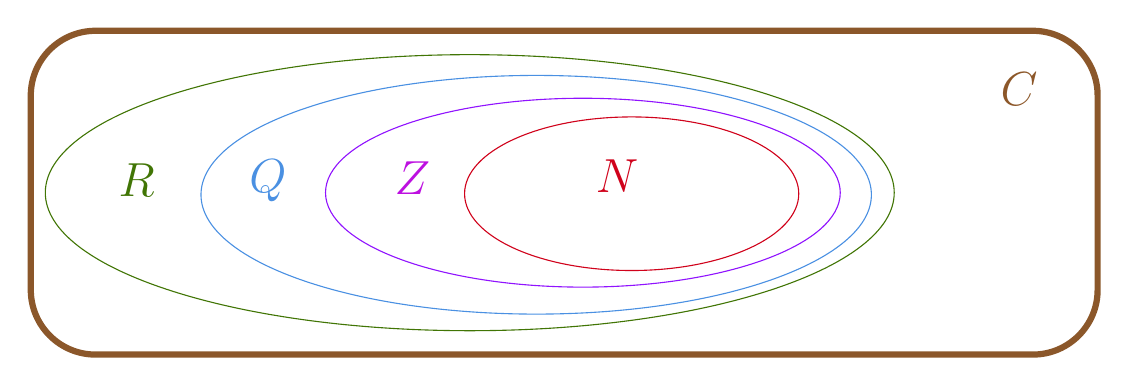
\begin{tikzpicture}[x=0.75pt,y=0.75pt,yscale=-1,xscale=1]
    %uncomment if require: \path (0,172); %set diagram left start at 0, and has height of 172
    
    %Shape: Ellipse [id:dp7922358117606259] 
    \draw  [color={rgb, 255:red, 208; green, 2; blue, 27 }  ,draw opacity=1 ] (230,92) .. controls (230,71.57) and (266.04,55) .. (310.5,55) .. controls (354.96,55) and (391,71.57) .. (391,92) .. controls (391,112.43) and (354.96,129) .. (310.5,129) .. controls (266.04,129) and (230,112.43) .. (230,92) -- cycle ;
    %Shape: Ellipse [id:dp27778820345068733] 
    \draw  [color={rgb, 255:red, 144; green, 19; blue, 254 }  ,draw opacity=1 ] (163,91.5) .. controls (163,66.37) and (218.52,46) .. (287,46) .. controls (355.48,46) and (411,66.37) .. (411,91.5) .. controls (411,116.63) and (355.48,137) .. (287,137) .. controls (218.52,137) and (163,116.63) .. (163,91.5) -- cycle ;
    %Shape: Ellipse [id:dp2930830644400444] 
    \draw  [color={rgb, 255:red, 74; green, 144; blue, 226 }  ,draw opacity=1 ] (103,92.5) .. controls (103,60.74) and (175.31,35) .. (264.5,35) .. controls (353.69,35) and (426,60.74) .. (426,92.5) .. controls (426,124.26) and (353.69,150) .. (264.5,150) .. controls (175.31,150) and (103,124.26) .. (103,92.5) -- cycle ;
    %Shape: Ellipse [id:dp715353025232164] 
    \draw  [color={rgb, 255:red, 65; green, 117; blue, 5 }  ,draw opacity=1 ] (28,91.5) .. controls (28,54.77) and (119.56,25) .. (232.5,25) .. controls (345.44,25) and (437,54.77) .. (437,91.5) .. controls (437,128.23) and (345.44,158) .. (232.5,158) .. controls (119.56,158) and (28,128.23) .. (28,91.5) -- cycle ;
    %Rounded Rect [id:dp4008700042872797] 
    \draw  [color={rgb, 255:red, 139; green, 87; blue, 42 }  ,draw opacity=1 ][line width=2.25]  (21,44.7) .. controls (21,27.47) and (34.97,13.5) .. (52.2,13.5) -- (503.8,13.5) .. controls (521.03,13.5) and (535,27.47) .. (535,44.7) -- (535,138.3) .. controls (535,155.53) and (521.03,169.5) .. (503.8,169.5) -- (52.2,169.5) .. controls (34.97,169.5) and (21,155.53) .. (21,138.3) -- cycle ;
    
    % Text Node
    \draw (292,74.4) node [anchor=north west][inner sep=0.75pt]  [font=\LARGE,color={rgb, 255:red, 208; green, 2; blue, 27 }  ,opacity=1 ]  {$\mathbb{N}$};
    % Text Node
    \draw (195,75.4) node [anchor=north west][inner sep=0.75pt]  [font=\LARGE,color={rgb, 255:red, 189; green, 16; blue, 224 }  ,opacity=1 ]  {$\mathbb{Z}$};
    % Text Node
    \draw (125,74.4) node [anchor=north west][inner sep=0.75pt]  [font=\LARGE,color={rgb, 255:red, 74; green, 144; blue, 226 }  ,opacity=1 ]  {$\mathbb{Q}$};
    % Text Node
    \draw (62,76.4) node [anchor=north west][inner sep=0.75pt]  [font=\LARGE,color={rgb, 255:red, 65; green, 117; blue, 5 }  ,opacity=1 ]  {$\mathbb{R}$};
    % Text Node
    \draw (487,32.4) node [anchor=north west][inner sep=0.75pt]  [font=\LARGE,color={rgb, 255:red, 139; green, 87; blue, 42 }  ,opacity=1 ]  {$\mathbb{\textcolor[rgb]{0.55,0.34,0.16}{C}}$};
    
    
    \end{tikzpicture}
\end{image}    

% insert venndiagram (middelgroot)

insert reëele rechte 


%voorlopig hebben we hier niet de opbouw van de verschillende venndiagrammen etc. 
% Indien dit erg goed is kunnen we die wel nog invoegen opzich. 


In het vierde jaar heb je geleerd hoe je de tweedegraadsvergelijking \(ax^2 + bx + c = 0\) kan oplossen. 
Hierbij maakte je een onderscheid naargelang het teken van de discriminant \(D = b^2 - 4ac\).
De vergelijking \(x^2 + 2x + 5 = 0\) heeft als discriminant \(D = b^2 - 4ac = 4 - 20 = -16\). 
De discriminant is negatief en deze vergelijking heeft dus geen oplossingen. 
De grafiek van deze functie heeft geen snijpunten met de x-as. (tikzpicture invoegen)

Je hebt geleerd dat de algemene oplossing voor een tweedegraadsvergelijking gegeven wordt door 
\[  
    x_{1,2} = \frac{-b +- \sqrt{D}}{2a}. 
\]
Misschien is de formule toch zinvol? Rekenen met de negatieve discriminant geeft:

\[ x_{1,2} = \frac{-2 +- \sqrt{-16}}{2} = \frac{-2 +- 4\sqrt{-1}}{2} = -1 +- 2\sqrt{-1}\]. 

In deze 'mogelijke oplossing' staat \(\sqrt{-1}\). Omdat er geen reëel getal is met als vierkantswortel -1, is er voor deze vergelijking geen oplossing in \(\R\). In de uitbreiding van de natuurlijke getallen \(N\) tot de reële getallen \(R\) werd de verzameling getallen telkens uitgebreid als er geen oplossing was. In dit hoofdstuk worden de reële getallen \(\R\) uitgebreid door een nieuw getal \(i\) toe te voegen met de eigenschap dat \(i^2 = -1\). Dit zijn de complexe getallen \(\C\). De tweedegraadsvergelijking \(x^2 + 2x + 5 = 0\) heeft dan wel oplossingen in de complexe getallen: \(-1 + 2i\)  en  \(-1-2i\).



\end{document}